Spoofax is a platform that allows for giving a completely
\emph{declarative} definition of a programming language and accompanying
IDE support~\cite{Kats10a}. Such a platform is called a \emph{language
workbench}. The definition of a programming language is done using
high-level \emph{meta-languages} for each aspect of the programming
language.

To define a language declaratively means that one uses the
meta-languages to specify \emph{what} the properties of a language are, not
\emph{how} these properties are implemented. For example, instead of asking
\emph{​``How do I implement a tokenizer and parser for my language?''​}, one
asks \emph{​``What is the syntax of my language?''​}. From such a description
in a meta-language, the tokenizer and parser can be derived without
the designer of the language ever having to care about its
implementation.

This section goes over the elements that make up the specification of
a language, and for each element the relevant part of Spoofax is
given\footnote{This section follows the structure of the
language specification portion of the compiler construction course at
the TU Delft. The slides can be found here:
\url{http://tudelft-in4303.github.io/lectures/specification/}.}. The parts
of a language specification are:

\begin{enumerate}
\item \hyperref[sec:syntax-def]{Syntax Definition}: Specifying the syntax of a language.
\item \hyperref[sec:static-analysis]{Static Semantics}: Describing the static analysis part of a
language (type checking, name binding and variable scoping).
\item \hyperref[sec:term-rewrite]{Term Rewriting and Program Transformation}: Rewriting abstract
syntax trees (ASTs) to new ASTs, for example to declare desugaring
rules.
\item \hyperref[sec:dynamic-semantics]{Dynamic Semantics}: Defining what the language does upon execution.
\end{enumerate}

After that, the section concludes with a description of \hyperref[sec:editor-serv]{Editor
Services in Spoofax}.
\subsection{Syntax Definition}
\label{sec:syntax-def}
The first part of the specification of a language is its syntax. The
syntax of a language is often specified by means of a \emph{lexical
grammar} and a \emph{context-free grammar}, as can be seen in the
specification of, for example, Standard ML~\cite{Milner97}. The
lexical grammar is most often defined using regular expressions. It
defines the individual words made up of characters, such as
identifiers and numeric constants. The context-free grammar then
defines syntactically valid sentences made up of words.

\subsubsection{SDF3: syntax definition in Spoofax}
\label{sec:orgheadline1}
To specify a syntax definition declaratively in Spoofax, a domain
specific language (DSL) called \emph{SDF3}~\cite{Vollebregt12} is used.
SDF3 is the third generation of the \emph{Syntax Definition Formalism}
(SDF)~\cite{Heering89}. It uses only context-free grammer
productions for the specification of both the lexical syntax and the
context-free syntax, a feature that was introduced in
SDF2~\cite{Visser97}.

The declarative nature of SDF3 allows for thinking in terms of the
structure (the \emph{what}), instead of in terms of parser algorithms (the
\emph{how}) as is the case with many current parsing
algorithms~\cite{Kats10b}. The syntax definition is used to make
parsers that parse a textual representation of a program into its AST,
and pretty-printers for mapping ASTs back to text. However, due to its
declarative nature, SDF3 is not limited to generating parsers and
pretty printers: it can also be used for error recovery
rules~\cite{deJonge12}, syntax highlighting rules and folding
rules for editors (see section \ref{sec:editor-serv}).

All of the other parts of Spoofax use the AST that is produced by a
parser generated from an SDF3 specification.
\subsection{Static Semantics}
\label{sec:static-analysis}
Static semantics refer to the meaning of what a well-formed program is
for a particular language~\cite{Milner97}. This imposes more
constraints than syntax definition, such as name binding, scoping
rules, and type checking. These cannot be specified by a syntax
definition alone, and are thus considered separately.
\subsubsection{Declarative static semantics specification in Spoofax}
\label{sec:orgheadline2}
In Spoofax, all the static semantics as well as the dynamic semantics
used to be specified with the \emph{Stratego} transformation language
(which is discussed in section \ref{sec:term-rewrite}). Nowadays, two
high-level DSLs exist for specifying static semantics declaratively:
NaBL and TS. The two DSLs can work together: for instance, the type of
a variable can be set with NaBL, so that TS can be used to make
assertions on the type of that variable.
\subsubsection{NaBL: the Name Binding Language}
\label{sec:nabl}
With \emph{NaBL} (pronounced \emph{enable}), name binding and scoping rules can
be specified declaratively~\cite{KonatKWV12}. Here is an example
of the name binding and scoping rules for a class, from the \emph{paplj}
language\footnote{paplj is used as an exercise language for the
``Declare Your Language'' book, which is a work-in-progress at the time
of writing. More information can be found here:
\url{https://github.com/MetaBorgCube/declare-your-language}}
\lstset{language=nabl,numbers=left}
\begin{lstlisting}
namespaces Program Class Field Method Variable
// ...
binding rules
  Class(c, _, _, _) :
    defines Class c of type ClassT(c)
    // Declare new scope
    scopes Field, Method, Variable
    implicitly defines Variable This() of type ClassT(c)

  Extends(c) :
    // Import namespaces from superclass
    imports Field, Method from Class c
\end{lstlisting}
The first line declares the \emph{namespaces} to consider. A namespace is a
way to distinguish different kinds of
names~\cite{KonatKWV12}. Then for each node in the AST resulting
from the parsing, for example a \texttt{Class} node, the name binding and
scoping rules can be defined. In the example, each \texttt{Class} node
declares a new scope for its fields, methods and variables. It also
implicitly defines the \texttt{this} variable. The \texttt{Extends} node can then
import the fields and methods into its scope.

As can be seen from line 8, it can also associate type information
with names to interplay with TS. The type annotations can also be used
for instance when desugaring or rewriting with Stratego (see section
\ref{sec:term-rewrite}).
\subsubsection{TS: the Type Specification language}
\label{sec:orgheadline3}
Type checking can be done by specifying typing rules with the \emph{TS}
DSL. Again an example of the paplj language:
\lstset{language=type-spec,numbers=left}
\begin{lstlisting}
type rules
  Class(c1, Extends(c2), _, _) :-
    where store ClassT(c1) <sub: ClassT(c2)

  x@This() : t
    where definition of x : t
// ...
type rules
  Add(e1, e2) : NumT()
    where e1 : NumT() else error "number expected" on e1
      and e2 : NumT() else error "number expected" on e2
\end{lstlisting}
Rules can recursively set constraints on AST-nodes, such as the \texttt{Add}
node in the above example.

Again, in line 5, interplay can be seen between TS an NaBL. Here the
type of a variable can be accessed, which is set in the NaBL
specification (see the previous section \ref{sec:nabl}).
\subsection{Term Rewriting and Program Transformation}
\label{sec:term-rewrite}
Spoofax offers a high level declarative DSL called \emph{Stratego} for
program transformation~\cite{Visser01}. Stratego operates on ASTs,
and is the most general part of Spoofax: it can be used for specifying
the static semantics (name binding, type checking), desugaring rules
and the dynamic semantics of a language. As the static semantics can
now be done using NaBL and TS, and the dynamic semantics with DynSem
(section \ref{sec:dynamic-semantics}), Stratego is now used to specify
desugaring rules for a language, as well as optimizations such as
constant folding and other applications of AST transformations.

Stratego is based on the notions of \emph{term rewrite rules} and so-called
\emph{strategies}.
\subsubsection{Term rewrite rules}
\label{sec:orgheadline4}
A rewrite rule is a transformation on a term, in which the left-hand
side allows for pattern matching and variable binding, and the right
hand side instantiates new replacement terms. An example of a rewrite
rule for paplj is given below.
\lstset{language=stratego,numbers=left}
\begin{lstlisting}
rules
  desugar-let :
  	Let([], e) -> e

  desugar-let :
  	Let([b1, b2 | bs], e) -> Let([b1], Let([b2 | bs], e))
\end{lstlisting}
This desugars a \texttt{let} expression with multiple bindings into multiple
nested \texttt{let} expressions each having just one binding.
\subsubsection{Strategies}
\label{sec:orgheadline5}
Strategies are used to select and apply term rewrite rules, to
construct the main algorithm of the program transformation. One can
use multiple combinators to compose rewrite rules and other
strategies. Another example from paplj is given below:
\lstset{language=stratego,numbers=left}
\begin{lstlisting}
strategies
  pre-desugar =
    innermost(desugar-let <+ desugar-do)

  post-desugar =
    innermost(desugar-do <+ desugar-get <+ desugar-set);
    resugar
\end{lstlisting}
For example, the strategy \texttt{innermost} is used to apply the strategy
given as parameter (a composition of rewrite rules) in a specific
traversal order on the AST nodes.
\subsection{Dynamic Semantics}
\label{sec:dynamic-semantics}
Dynamic semantics refers to how a program written in some language
behaves~\cite{Winskel93}. There are multiple approaches to
formally specify the dynamic semantics of a programming language (for
an extensive treatment, see~\cite{Winskel93}). For this section
only one sort of approach is relevant, namely \emph{rule-based operational}
\emph{semantics} (see~\cite{Plotkin04} for a historical account of this
approach).

\subsubsection{DynSem: rule-based dynamic semantics}
\label{ssec:dynsem}
In Spoofax, the dynamic semantics of a language used to be specified
with Stratego. However, the Spoofax team has developed a more
high-level method to declare the dynamic semantics of a language,
namely a DSL called \emph{DynSem}~\cite{VerguNV15}. As with all DSLs in
Spoofax, DynSem offers a declarative approach to generate the
\emph{implementation} out of the \emph{specification}. Indeed, from a DynSem
specification of a language, an interpreter for that language can be
generated.

In DynSem, the dynamic semantics are specified by means of rules. To
show how rules can define the dynamic semantics of a language,
consider the classic example of the \(\beta\)-reduction, which defines
function application in the lambda calculus. The rule replaces all the
occurences of the parameter \(x\) with the argument \(e_2\), within the
expression \(e_1\):

\begin{equation}
(\lambda x.e_1) e_2 \rightarrow e_1[x := e_2]
\end{equation}

In a similar way, dynamic semantics can be specified in DynSem, in a
syntax very similar to the formal syntax used in the literature. Take
here the example of defining method calling in paplj:
\lstset{language=dynsem,numbers=left}
\begin{lstlisting}
rules
  // ...
  Call(o, m, vs: List(V)) --> v'
    where lookupMethod(o, m) --> Method(_, _, params, e);
          This o, Env bindVars(params, vs) |- e --> v'.
\end{lstlisting}
The bottom line represents the rule of the method body, \(e\),
evaluating to the return value \(v'\), by binding the argument values to
the parameter in the environment and binding the \texttt{this} variable to
the object on which the method is called. Exactly how \(e\) evaluates to
\(v'\) is defined using other rules, which are left out in this example.
\lstset{numbers=none}

\subsection{Editor Services}
\label{sec:editor-serv}
This section concludes with a brief description of editor services,
which provide the IDE support for languages defined in
Spoofax. Examples of such services include an outline view, menus in
which one can bind actions to menu buttons (see figure
\ref{fig:menu-actions}), but also syntax highlighting and code folding
rules\footnote{More services are listed on the Spoofax
website: \url{http://www.metaborg.org/spoofax/editor-services/}}.

\begin{figure}[htb]
\centering
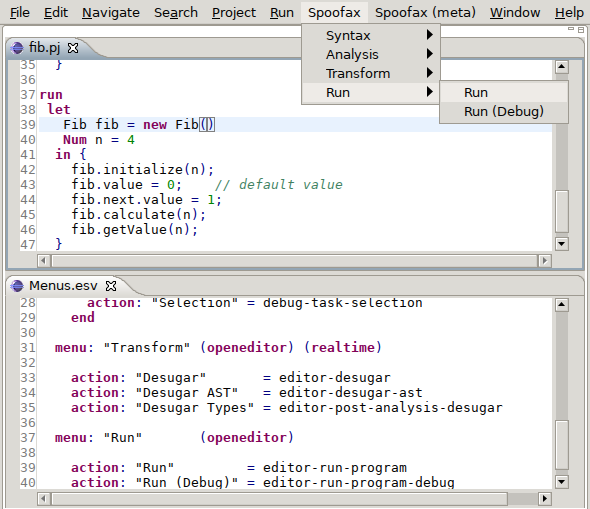
\includegraphics[width=0.6\textwidth]{./img/menu-actions.png}
\caption{\label{fig:menu-actions}
A menu action for the paplj language defined using Spoofax. The bottom window shows the menu definition, the top window shows a program written in paplj.}
\end{figure}

Editor services are defined using a DSL, shown in the bottom window of
figure \ref{fig:menu-actions}. In the case of menus, their actions are
specified using Stratego, and via Stratego the actions can even be
specified in Java. As such, Spoofax allows for defining arbitrarily
complex IDE actions.

Many of these editor services such as syntax highlighting and code
folding rules can be derived from the syntax
definition~\cite{Kats10c}, and can be further customized if
needed. Taken together with the language definition, the editor
services provide a language with a complete and state-of-the-art IDE
experience~\cite{Kats10a}.
